%arborescence du site internet (quel page est relier avec laquelle...)
L'arborescence de notre site web est telle que nous pouvons accéder à chacune des pages grâce au menu du haut de page ("accueil", "actualités", "logements", "voyages") et le menu du bas de page ("mention légale", "contact", "réseaux sociaux").

\begin{figure}[h]
    \centering
    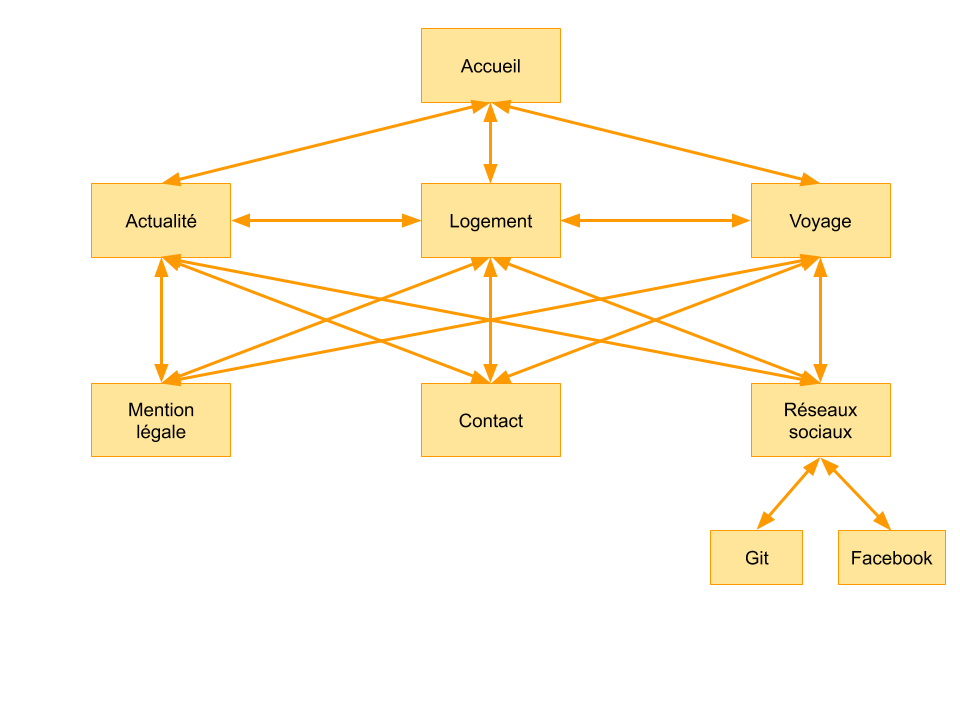
\includegraphics[scale=0.5]{arbo.png}
\end{figure}

Sans utiliser ces menus, il est possible depuis la page d'"accueil" d'être dirigé sur les pages "actualités", "logements" ou "voyages".
Depuis la page "mention légale" on peut accéder à celle des "réseaux sociaux", dans laquelle on peut aller sur le projet Git (pour télécharger les sources et le code LaTeX) et la page Facebook du projet. 

